\documentclass[]{informeutn}

% ---------------------------------------------------------------------------------------------------------------------
% Paquetes que no provee la clase (si informeutn.cls ya carga alguno, borrar la línea correspondiente)
% ---------------------------------------------------------------------------------------------------------------------
\usepackage{siunitx}
\usepackage{subcaption}
\usepackage{listings}
\usepackage[backend=bibtex, style=alphabetic, sorting=ynt]{biblatex}
\addbibresource{fuentes.bib}
\usetikzlibrary{calc}

\sisetup{
  output-decimal-marker={,},
  exponent-product=\cdot,
  separate-uncertainty=true,
}

\lstdefinestyle{ltspice}{
  backgroundcolor=\color{gray!10},
  basicstyle=\ttfamily\small,
  keywordstyle=\color{blue},
  frame=single,
  breaklines=true,
  captionpos=b
}

% ---------------------------------------------------------------------------------------------------------------------
% Metadatos de la carátula
% ---------------------------------------------------------------------------------------------------------------------
\materia{Teoría de Circuitos II}
\titulo{Trabajo Práctico N\textsuperscript{o} 2: Diseño de Filtros Activos}
\subtitulo{Filtro activo de señal de campo (4--20 mA) y diseño de filtros pasa bajos, pasa altos y pasa banda}
\comision{}                                     % TODO: completar comisión
\autores{Ernst, Pedro \\ Gil, Ignacio \\ Rao, Valentino}   % TODO: agregar legajos si la cátedra lo pide
\fecha{\today}

\begin{document}
  \maketitle
  \tableofcontents
  \setcounter{page}{1}
  \thispagestyle{plain}

  % Capítulos (un archivo por punto de la consigna)
  \chapter{Introducción}
\label{chap:introduccion}

\section{Objetivos}
\label{sec:objetivos}

\begin{itemize}
  \item Estudiar los conceptos básicos sobre el análisis y diseño de filtros activos.
  \item Aplicar las técnicas explicadas en clase para el cálculo de filtros activos.
  \item Implementar filtros activos.
\end{itemize}

\section{Descripción del trabajo práctico}
\label{sec:descripcion}

El trabajo práctico se divide en dos actividades. La primera (capítulo~\ref{chap:senal-campo}) consiste en el diseño
e implementación de un módulo de filtrado activo para una señal de campo de $\SI{4}{\milli\ampere}$ a
$\SI{20}{\milli\ampere}$, compuesto por un amplificador de instrumentación, un filtro pasa bajos Sallen-Key de
segundo orden y un convertidor tensión-corriente, todo alimentado con una fuente simple de $\SI{24}{\volt}$.

La segunda actividad (capítulos~\ref{chap:pasa-bajos} a~\ref{chap:pasa-banda}) consiste en el diseño de tres filtros
con los parámetros asignados al grupo, resumidos en la tabla~\ref{tab:asignacion}. Para cada uno se realizan los
cálculos, las simulaciones con elementos ideales y con valores comerciales, y para dos de ellos la implementación
física y el relevamiento de la respuesta en frecuencia.

\begin{table}[!ht]
  \centering
  \resizebox{\textwidth}{!}{\begin{tabular}{|l|c|c|c|c|c|c|}
    \hline
    Filtro & Orden & $A_{max}$ [dB] & $f_p$ / $f_o$ [kHz] & $BW$ [kHz] & Ganancia [V/V] & Aproximación / Topología \\
    \hline
    Pasa bajos & 4 & 1,5  & 5,5 & --  & 4    & Butterworth / Sallen-Key \\
    Pasa altos & 4 & 2,25 & 33  & --  & 12,5 & Butterworth / Sallen-Key \\
    Pasa banda & 2 & 0,1  & 28  & 1,7 & 9    & Butterworth / Sallen-Key \\
    \hline
  \end{tabular}}
  \caption{Parámetros asignados al Grupo 2.}
  \label{tab:asignacion}
\end{table}

% TODO: indicar cuáles dos filtros se implementan físicamente y cuál queda para el TP de filtros digitales.

  \chapter{Filtro activo de señal de campo}
\label{chap:senal-campo}

\section{Objetivos}
\label{sec:campo-objetivos}

\begin{itemize}
  \item Diseñar e implementar un filtro activo pasa bajos analógico para eliminar ruido de modo común y de alta
    frecuencia en líneas de instrumentación de gran longitud ($\SI{10}{\metre}$).
  \item Comprender el funcionamiento de un receptor diferencial y un convertidor tensión-corriente (V $\rightarrow$ I).
  \item Realizar la caracterización estática y dinámica del circuito mediante instrumental de laboratorio.
\end{itemize}

\section{Planteo del problema}
\label{sec:campo-planteo}

En un entorno industrial, un sensor transmite una variable de proceso mediante un bucle de
$\SI{4}{\milli\ampere}$ a $\SI{20}{\milli\ampere}$. El cable de interconexión recorre $\SI{10}{\metre}$ junto a
líneas de potencia, acoplando ruido de la red eléctrica ($\SI{50}{\hertz}$) y de conmutación de motores. Para que la
señal pueda ser procesada por la entrada analógica diferencial de corriente de un PLC, se diseña un módulo
intermedio de filtrado activo alimentado con la fuente industrial de $\SI{24}{\volt}$, compuesto por las tres etapas
en cascada de la figura~\ref{fig:diagrama-bloques}.

\begin{figure}[!ht]
  \centering
  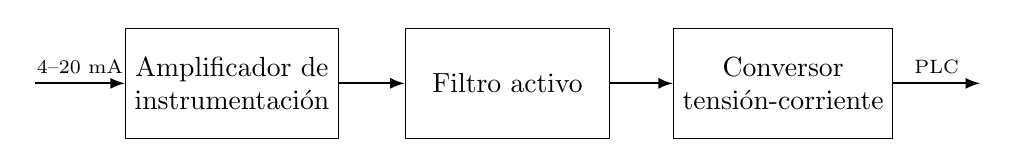
\begin{tikzpicture}[
    bloque/.style={draw, minimum width=2.6cm, minimum height=1.4cm, align=center},
    flecha/.style={->, >=latex, thick},
  ]
  \node[bloque] (e1) at (0,0) {Amplificador de\\instrumentación};
  \node[bloque] (e2) at (3.5,0) {Filtro activo};
  \node[bloque] (e3) at (7,0) {Conversor\\tensión-corriente};
  \draw[flecha] (-2.5,0) -- (e1) node[midway, above] {\scriptsize 4--20 mA};
  \draw[flecha] (e1) -- (e2);
  \draw[flecha] (e2) -- (e3);
  \draw[flecha] (e3) -- (9.5,0) node[midway, above] {\scriptsize PLC};
\end{tikzpicture}

  \caption{Diagrama en bloques del módulo de filtrado.}
  \label{fig:diagrama-bloques}
\end{figure}

\section{Especificaciones del circuito}
\label{sec:campo-especificaciones}

\subsection{Alimentación}
\label{subsec:campo-alimentacion}

Todo el módulo se alimenta con una fuente simple de $\SI{24}{\volt}$, sin tensión negativa. Por este motivo se
utiliza el LM324, cuyo rango de modo común de entrada incluye $\SI{0}{\volt}$ y cuya salida puede acercarse a masa.
El circuito completo requiere cinco amplificadores operacionales, por lo que se emplean dos integrados LM324:

\begin{itemize}
  \item U1A, U1B y U1C: etapa 1 (amplificador de instrumentación).
  \item U1D: etapa 2 (filtro Sallen-Key).
  \item U2A: etapa 3 (convertidor V $\rightarrow$ I). Las secciones U2B a U2D se conectan como seguidor con la entrada
    no inversora a masa.
\end{itemize}

El pin 4 de cada integrado se conecta a $\SI{+24}{\volt}$ y el pin 11 a GND, con un capacitor de desacople de
$\SI{100}{\nano\farad}$ lo más cerca posible de cada integrado.

% TODO: justificar brevemente por qué el TL084 no es apto con fuente simple (rango de entrada y excursión de salida).

\subsection{Etapa 1: receptor diferencial e instrumentación (I \texorpdfstring{$\rightarrow$}{->} V)}
\label{subsec:campo-etapa1}

La configuración de la etapa 1 se muestra en la figura~\ref{crkt:etapa1}. La resistencia de shunt flotante
$R_{shunt\_in} = \SI{250}{\ohm}$ convierte los $\SI{4}{\milli\ampere}$ a $\SI{20}{\milli\ampere}$ en una tensión
diferencial de $\SI{1}{\volt}$ a $\SI{5}{\volt}$. La resistencia $R_{CM} = \SI{1}{\mega\ohm}$ fija el modo común del
bucle flotante y provee el camino de polarización de las entradas. Los seguidores U1A y U1B evitan que la resistencia
de entrada del restador ($R_3 + R_4 = \SI{20}{\kilo\ohm}$) cargue al shunt, lo que produciría un error de ganancia de
$\SI{-1.23}{\percent}$. El restador U1C tiene ganancia unitaria con $R_3 = R_4 = R_5 = R_f = \SI{10}{\kilo\ohm}$
(tolerancia $\SI{1}{\percent}$ o mejor), de modo que

\begin{equation}
  V_{E1} = V_{(+)} - V_{(-)} = I_{in} \cdot R_{shunt\_in}
  \label{eq:ve1}
\end{equation}

\begin{figure}[!ht]
  \centering
  \begin{tikzpicture}[american, scale=0.9]
  % Operacionales
  \node[op amp] (u1a) at (5.2,3) {\scriptsize U1A};
  \node[op amp, noinv input up] (u1b) at (5.2,0) {\scriptsize U1B};
  \node[op amp] (u1c) at (10.6,1.5) {\scriptsize U1C};

  % Lazo (-) y (+)
  \draw (0,3.5) node[ocirc, label=left:{Lazo $(-)$}] {} to[short] (1.4,3.5) node[circ] {}
    to[short, -*] (3,3.5) -| (u1a.+);
  \draw (0,0) node[ocirc, label=left:{Lazo $(+)$}] {} to[short, i=$I_{in}$] (1.4,0) node[circ] {} -| (u1b.+);

  % Shunt y referencia de modo común
  \draw (1.4,3.5) to[R, l_=\shortstack{$R_{shunt\_in}$\\\SI{250}{\ohm}}] (1.4,0);
  \draw (3,3.5) to[R, l_=\shortstack{$R_{CM}$\\\SI{1}{\mega\ohm}}] (3,1.8) node[ground] {};

  % Seguidores
  \draw (u1a.out) -- ++(0.4,0) coordinate (ao);
  \draw (ao) -- ++(0,1.3) -| (u1a.-);
  \draw (u1b.out) -- ++(0.4,0) coordinate (bo);
  \draw (bo) -- ++(0,-1.3) -| (u1b.-);

  % Restador
  \draw (ao) node[circ] {} -- (ao |- u1c.-) to[R, l=\shortstack{$R_3$\\\SI{10}{\kilo\ohm}}] ($(u1c.-)+(-0.4,0)$)
    node[circ] (nm) {} -- (u1c.-);
  \draw (bo) node[circ] {} -- (bo |- u1c.+) to[R, l_=\shortstack{$R_4$\\\SI{10}{\kilo\ohm}}] ($(u1c.+)+(-0.4,0)$)
    node[circ] (np) {} -- (u1c.+);
  \draw (np) to[R, l=\shortstack{$R_5$\\\SI{10}{\kilo\ohm}}] ++(0,-2.6) node[ground] {};
  \draw (u1c.out) -- ++(0.4,0) coordinate (co) node[circ] {} -- ++(0,1.6) coordinate (ft);
  \draw (ft) to[R, l=$R_f$, a=\SI{10}{\kilo\ohm}] (ft -| nm) -- (nm);
  \draw (co) to[short, -o] ++(0.9,0) node[right, align=left] {$V_{E1}$\\\scriptsize 1--5 V};
\end{tikzpicture}

  \caption{Etapa 1: amplificador de instrumentación de ganancia unitaria.}
  \label{crkt:etapa1}
\end{figure}

\subsection{Etapa 3: convertidor tensión-corriente (V \texorpdfstring{$\rightarrow$}{->} I)}
\label{subsec:campo-etapa3}

La salida del filtro se reinyecta como corriente a la entrada analógica del PLC mediante una fuente de corriente tipo
sumidero con transistor NPN (figura~\ref{crkt:etapa3}). El operacional U2A fuerza la tensión de emisor a ser igual a
$V_{filtro}$, por lo que la corriente de salida resulta

\begin{equation}
  I_{out} = \alpha \, \frac{V_{filtro}}{R_{shunt\_out}} \approx \frac{V_{filtro}}{\SI{250}{\ohm}}
  \label{eq:iout}
\end{equation}

de modo que los $\SI{1}{\volt}$ a $\SI{5}{\volt}$ del filtro se convierten en $\SI{4}{\milli\ampere}$ a
$\SI{20}{\milli\ampere}$, donde $\alpha = \beta / (\beta + 1)$. Con $\beta \approx$ 100 a 200 el error por
corriente de base es de $\SI{-0.5}{\percent}$ a $\SI{-1}{\percent}$, y debe tenerse en cuenta en el análisis de
error de la caracterización estática.

\begin{figure}[!ht]
  \centering
  \begin{tikzpicture}[american]
  \node[op amp, noinv input up] (u2a) at (3,0) {\scriptsize U2A};
  \node[npn] (q1) at (7.5,0) {};
  \node[anchor=west] at ($(q1.C)+(0.1,-0.4)$) {\scriptsize Q1 (BC337)};

  % Entrada
  \draw (0,0.5) node[ocirc, label={[align=left]left:$V_{filtro}$\\\scriptsize 1--5 V}] {} -- (u2a.+);

  % Base
  \draw (u2a.out) to[R, l=$R_B$, a=\SI{1}{\kilo\ohm}] (q1.B);

  % Colector: carga (PLC) y +24 V
  \draw (q1.C) to[R, l=$R_{carga}$ (PLC), a=\SI{250}{\ohm}, i<=$I_{out}$] ++(0,2.8) node[vcc] {$\SI{+24}{\volt}$};

  % Emisor: shunt de salida y realimentación
  \draw (q1.E) -- ++(0,-0.5) node[circ] (fb) {} to[R, l=$R_{shunt\_out}$, a=\SI{250}{\ohm}] ++(0,-2.2)
    node[ground] {};
  \draw (fb) -- (1.3,0 |- fb) -- (1.3,0 |- u2a.-) -- (u2a.-);
\end{tikzpicture}

  \caption{Etapa 3: convertidor tensión-corriente.}
  \label{crkt:etapa3}
\end{figure}

% TODO: verificación de márgenes a 20 mA: caída en R_shunt_out y R_carga, V_CE y P_D del BC337.

\section{Diseño del filtro activo}
\label{sec:campo-diseno}

\subsection{Cálculo matemático}
\label{subsec:campo-calculo}

Se diseña un filtro pasa bajos Sallen-Key de segundo orden con aproximación Butterworth y ganancia unitaria en la
banda de paso, con frecuencia de corte $f_c = \SI{10}{\hertz}$ ($\SI{-3}{\decibel}$). La función de transferencia
buscada es

\begin{equation}
  H(s) = \frac{\omega_0^2}{s^2 + \dfrac{\omega_0}{Q} s + \omega_0^2}
  \qquad \text{con } Q = \frac{1}{\sqrt{2}} \text{ y } \omega_0 = 2 \pi f_c
  \label{eq:campo-hs}
\end{equation}

Para la topología Sallen-Key de ganancia unitaria de la figura~\ref{crkt:sk-unitario} se tiene

\begin{align*}
  \omega_0 &= \frac{1}{\sqrt{R_1 R_2 C_1 C_2}} \\
  Q &= \frac{\sqrt{R_1 R_2 C_1 C_2}}{C_2 \left( R_1 + R_2 \right)}
\end{align*}

% TODO: desarrollar el cálculo (p. ej. R_1 = R_2 = R, C_1 = 2 C_2 para Q = 1/sqrt(2)) y obtener los valores teóricos.

\begin{figure}[!ht]
  \centering
  \begin{tikzpicture}[american]
  \node[op amp, noinv input up] (oa) at (6,0) {\scriptsize U1D};

  \draw (0,0.5) node[ocirc, label=left:$V_{E1}$] {} to[R, l=$R_1$] (1.8,0.5) node[circ] (n1) {}
    to[R, l=$R_2$] (3.6,0.5) node[circ] (n2) {} -- (oa.+);
  \draw (n2) to[C, l_=$C_2$] ++(0,-2) node[ground] {};
  \draw (oa.out) -- ++(0.6,0) node[circ] (out) {} to[short, -o] ++(1,0) node[right] {$V_{filtro}$};
  \draw (n1) to[C, l=$C_1$] ++(0,2) -| (out);
  \draw (oa.-) -- ++(-0.5,0) |- ($(oa.south)+(0,-0.6)$) -| (out);
\end{tikzpicture}

  \caption{Etapa 2: filtro pasa bajos Sallen-Key de ganancia unitaria.}
  \label{crkt:sk-unitario}
\end{figure}

\subsection{Selección de componentes}
\label{subsec:campo-componentes}

% TODO: proponer valores comerciales normalizados (serie E12/E24), recalcular f_c y Q resultantes y justificar el
% uso de capacitores de poliéster o film (no electrolíticos).

\begin{table}[!ht]
  \centering
  \begin{tabular}{|l|c|c|}
    \hline
    Componente & Valor calculado & Valor comercial \\
    \hline
    $R_1$ & & \\
    $R_2$ & & \\
    $C_1$ & & \\
    $C_2$ & & \\
    \hline
  \end{tabular}
  \caption{Valores calculados y comerciales del filtro Sallen-Key.}
  \label{tab:campo-componentes}
\end{table}

\subsection{Simulación}
\label{subsec:campo-simulacion}

% TODO: simular el circuito completo (etapa 1 + filtro + etapa 3), incluir el diagrama de Bode y verificar
% analíticamente la atenuación a 50 Hz. Guardar el proyecto de simulación en sources/.

\section{Implementación}
\label{sec:campo-implementacion}

% TODO: descripción del armado en protoboard (dos LM324 + BC337/2N2222), fotos en pictures/, y cómo se generó la
% señal de 4-20 mA para la caracterización estática (fuente + resistencia/potenciómetro) y dinámica (generador +
% resistencia serie).

\section{Mediciones}
\label{sec:campo-mediciones}

\subsection{Caracterización estática (linealidad)}
\label{subsec:campo-estatica}

\begin{table}[!ht]
  \centering
  \begin{tabular}{|c|c|c|c|c|}
    \hline
    $I_{in}$ [mA] & $V_{E1}$ [V] & $V_{filtro}$ [V] & $I_{out}$ [mA] & Error [\%] \\
    \hline
    4  & & & & \\
    8  & & & & \\
    12 & & & & \\
    16 & & & & \\
    20 & & & & \\
    \hline
  \end{tabular}
  \caption{Caracterización estática del módulo.}
  \label{tab:campo-estatica}
\end{table}

% TODO: graficar la curva de transferencia I_out vs I_in y calcular el error porcentual por tolerancias.

\subsection{Caracterización dinámica (respuesta en frecuencia)}
\label{subsec:campo-dinamica}

\begin{table}[!ht]
  \centering
  \begin{tabular}{|c|c|c|c|}
    \hline
    $f$ [Hz] & $V_{in,pp}$ [V] & $V_{out,pp}$ [V] & $|H|$ [dB] \\
    \hline
    1   & & & \\
    2   & & & \\
    5   & & & \\
    10  & & & \\
    20  & & & \\
    50  & & & \\
    100 & & & \\
    \hline
  \end{tabular}
  \caption{Barrido en frecuencia del módulo (señal senoidal con offset de continua).}
  \label{tab:campo-dinamica}
\end{table}

% TODO: determinar la frecuencia de corte real a -3 dB y la atenuación exacta a 50 Hz; comparar con la simulación.

  \chapter{Filtro pasa bajos}
\label{chap:pasa-bajos}

\section{Especificaciones}
\label{sec:pb-especificaciones}

\begin{table}[!ht]
  \centering
  \begin{tabular}{|l|c|}
    \hline
    Parámetro & Valor \\
    \hline
    Orden & 4 \\
    Atenuación máxima en banda de paso $A_{max}$ & $\SI{1.5}{\decibel}$ \\
    Frecuencia de paso $f_p$ & $\SI{5.5}{\kilo\hertz}$ \\
    Ganancia en banda de paso & 4 V/V \\
    Aproximación & Butterworth \\
    Topología & Sallen-Key \\
    \hline
  \end{tabular}
  \caption{Especificaciones del filtro pasa bajos.}
  \label{tab:pb-especificaciones}
\end{table}

\section{Diseño}
\label{sec:pb-diseno}

\subsection{Frecuencia de corte y polos de la aproximación}
\label{subsec:pb-polos}

Para un Butterworth de orden $n$, la atenuación en banda de paso vale $A_{max}$ en $f_p$, por lo que la frecuencia de
corte a $\SI{-3}{\decibel}$ se obtiene de

\begin{equation}
  f_c = \frac{f_p}{\left( 10^{A_{max}/10} - 1 \right)^{1/(2n)}}
  \label{eq:pb-fc}
\end{equation}

% TODO: calcular f_c, listar los pares de polos del Butterworth de orden 4 (Q_1 = 0,5412 y Q_2 = 1,3066) y repartir la
% ganancia total de 4 V/V entre las dos etapas.

\subsection{Cálculo de las etapas Sallen-Key}
\label{subsec:pb-etapas}

Cada etapa de segundo orden (figura~\ref{crkt:sk-pasa-bajos}) tiene ganancia $K = 1 + R_b / R_a$ y

\begin{align*}
  \omega_0 &= \frac{1}{\sqrt{R_1 R_2 C_1 C_2}} \\
  Q &= \frac{\sqrt{R_1 R_2 C_1 C_2}}{R_1 C_2 + R_2 C_2 + R_1 C_1 \left( 1 - K \right)}
\end{align*}

\begin{figure}[!ht]
  \centering
  \begin{tikzpicture}[american]
  \node[op amp, noinv input up] (oa) at (6,0) {};

  \draw (0,0.5) node[ocirc, label=left:$V_i$] {} to[R, l=$R_1$] (1.8,0.5) node[circ] (n1) {}
    to[R, l=$R_2$] (3.6,0.5) node[circ] (n2) {} -- (oa.+);
  \draw (n2) to[C, l_=$C_2$] ++(0,-2) node[ground] {};
  \draw (oa.out) -- ++(0.6,0) node[circ] (out) {} to[short, -o] ++(1,0) node[right] {$V_o$};
  \draw (n1) to[C, l=$C_1$] ++(0,2) -| (out);

  % Red de ganancia K = 1 + Rb/Ra
  \draw (oa.-) -- ++(-0.5,0) coordinate (m) -- ++(0,-1.1) node[circ] (m2) {}
    to[R, l=$R_a$] ++(0,-1.8) node[ground] {};
  \draw (m2) to[R, l_=$R_b$] (out |- m2) -- (out);
\end{tikzpicture}

  \caption{Etapa Sallen-Key pasa bajos de segundo orden con ganancia $K$.}
  \label{crkt:sk-pasa-bajos}
\end{figure}

% TODO: desarrollar el cálculo de R_1, R_2, C_1, C_2, R_a y R_b de cada etapa.

\subsection{Valores comerciales}
\label{subsec:pb-comerciales}

\begin{table}[!ht]
  \centering
  \begin{tabular}{|l|c|c|c|c|}
    \hline
     & \multicolumn{2}{c|}{Etapa 1} & \multicolumn{2}{c|}{Etapa 2} \\
    \cline{2-5}
    Componente & Calculado & Comercial & Calculado & Comercial \\
    \hline
    $R_1$ & & & & \\
    $R_2$ & & & & \\
    $C_1$ & & & & \\
    $C_2$ & & & & \\
    $R_a$ & & & & \\
    $R_b$ & & & & \\
    \hline
  \end{tabular}
  \caption{Valores calculados y comerciales del filtro pasa bajos.}
  \label{tab:pb-componentes}
\end{table}

\section{Simulación}
\label{sec:pb-simulacion}

\subsection{Función de transferencia con elementos ideales}
\label{subsec:pb-sim-ideal}

% TODO: diagrama de Bode (módulo y fase) con los valores calculados. Incluir el gráfico desde images/ o como pgfplots
% en figures/ (ver figures/bode-ejemplo.tex).

\subsection{Función de transferencia con valores comerciales}
\label{subsec:pb-sim-real}

% TODO: repetir con los valores comerciales y comparar f_c, A_max y ganancia obtenidas con las especificadas.

\section{Implementación y mediciones}
\label{sec:pb-mediciones}

% TODO: si este filtro es uno de los dos implementados: armado, fotos en pictures/, tabla de barrido en frecuencia,
% captura del perfil de frecuencia (FFT) del osciloscopio y comparación medido vs. simulado. Si no se implementa,
% indicar que se realiza en el TP de filtros digitales.

\begin{table}[!ht]
  \centering
  \begin{tabular}{|c|c|c|c|c|}
    \hline
    $f$ [kHz] & $V_{in,pp}$ [V] & $V_{out,pp}$ [V] & $|H|$ medido [dB] & $|H|$ simulado [dB] \\
    \hline
     & & & & \\
     & & & & \\
     & & & & \\
    \hline
  \end{tabular}
  \caption{Relevamiento de la respuesta en frecuencia del filtro pasa bajos.}
  \label{tab:pb-barrido}
\end{table}

  \chapter{Filtro pasa altos}
\label{chap:pasa-altos}

\section{Especificaciones}
\label{sec:pa-especificaciones}

\begin{table}[!ht]
  \centering
  \begin{tabular}{|l|c|}
    \hline
    Parámetro & Valor \\
    \hline
    Orden & 4 \\
    Atenuación máxima en banda de paso $A_{max}$ & $\SI{2.25}{\decibel}$ \\
    Frecuencia de paso $f_p$ & $\SI{33}{\kilo\hertz}$ \\
    Ganancia en banda de paso & 12,5 V/V \\
    Aproximación & Butterworth \\
    Topología & Sallen-Key \\
    \hline
  \end{tabular}
  \caption{Especificaciones del filtro pasa altos.}
  \label{tab:pa-especificaciones}
\end{table}

\section{Diseño}
\label{sec:pa-diseno}

\subsection{Frecuencia de corte y polos de la aproximación}
\label{subsec:pa-polos}

El filtro pasa altos se obtiene del prototipo pasa bajos normalizado mediante la transformación
$s \rightarrow \omega_0 / s$, por lo que la frecuencia de corte a $\SI{-3}{\decibel}$ queda por debajo de $f_p$:

\begin{equation}
  f_c = f_p \left( 10^{A_{max}/10} - 1 \right)^{1/(2n)}
  \label{eq:pa-fc}
\end{equation}

% TODO: calcular f_c, listar los polos del Butterworth de orden 4 (Q_1 = 0,5412 y Q_2 = 1,3066) y repartir la ganancia
% total de 12,5 V/V entre las dos etapas. Verificar el producto ganancia-ancho de banda del operacional elegido
% (ganancia por etapa x frecuencia máxima de interés).

\subsection{Cálculo de las etapas Sallen-Key}
\label{subsec:pa-etapas}

Cada etapa de segundo orden (figura~\ref{crkt:sk-pasa-altos}) tiene ganancia $K = 1 + R_b / R_a$ y

\begin{align*}
  \omega_0 &= \frac{1}{\sqrt{R_1 R_2 C_1 C_2}} \\
  Q &= \frac{\sqrt{R_1 R_2 C_1 C_2}}{R_2 C_1 + R_2 C_2 + R_1 C_2 \left( 1 - K \right)}
\end{align*}

\begin{figure}[!ht]
  \centering
  \begin{tikzpicture}[american]
  \node[op amp, noinv input up] (oa) at (6,0) {};

  \draw (0,0.5) node[ocirc, label=left:$V_i$] {} to[C, l=$C_1$] (1.8,0.5) node[circ] (n1) {}
    to[C, l=$C_2$] (3.6,0.5) node[circ] (n2) {} -- (oa.+);
  \draw (n2) to[R, l_=$R_2$] ++(0,-2) node[ground] {};
  \draw (oa.out) -- ++(0.6,0) node[circ] (out) {} to[short, -o] ++(1,0) node[right] {$V_o$};
  \draw (n1) to[R, l=$R_1$] ++(0,2) -| (out);

  % Red de ganancia K = 1 + Rb/Ra
  \draw (oa.-) -- ++(-0.5,0) coordinate (m) -- ++(0,-1.1) node[circ] (m2) {}
    to[R, l=$R_a$] ++(0,-1.8) node[ground] {};
  \draw (m2) to[R, l_=$R_b$] (out |- m2) -- (out);
\end{tikzpicture}

  \caption{Etapa Sallen-Key pasa altos de segundo orden con ganancia $K$.}
  \label{crkt:sk-pasa-altos}
\end{figure}

% TODO: desarrollar el cálculo de R_1, R_2, C_1, C_2, R_a y R_b de cada etapa.

\subsection{Valores comerciales}
\label{subsec:pa-comerciales}

\begin{table}[!ht]
  \centering
  \begin{tabular}{|l|c|c|c|c|}
    \hline
     & \multicolumn{2}{c|}{Etapa 1} & \multicolumn{2}{c|}{Etapa 2} \\
    \cline{2-5}
    Componente & Calculado & Comercial & Calculado & Comercial \\
    \hline
    $R_1$ & & & & \\
    $R_2$ & & & & \\
    $C_1$ & & & & \\
    $C_2$ & & & & \\
    $R_a$ & & & & \\
    $R_b$ & & & & \\
    \hline
  \end{tabular}
  \caption{Valores calculados y comerciales del filtro pasa altos.}
  \label{tab:pa-componentes}
\end{table}

\section{Simulación}
\label{sec:pa-simulacion}

\subsection{Función de transferencia con elementos ideales}
\label{subsec:pa-sim-ideal}

% TODO: diagrama de Bode (módulo y fase) con los valores calculados.

\subsection{Función de transferencia con valores comerciales}
\label{subsec:pa-sim-real}

% TODO: repetir con los valores comerciales y con el modelo real del operacional; comparar con las especificaciones.

\section{Implementación y mediciones}
\label{sec:pa-mediciones}

% TODO: si este filtro es uno de los dos implementados: armado, fotos en pictures/, tabla de barrido en frecuencia,
% captura del perfil de frecuencia (FFT) del osciloscopio y comparación medido vs. simulado. Si no se implementa,
% indicar que se realiza en el TP de filtros digitales.

\begin{table}[!ht]
  \centering
  \begin{tabular}{|c|c|c|c|c|}
    \hline
    $f$ [kHz] & $V_{in,pp}$ [V] & $V_{out,pp}$ [V] & $|H|$ medido [dB] & $|H|$ simulado [dB] \\
    \hline
     & & & & \\
     & & & & \\
     & & & & \\
    \hline
  \end{tabular}
  \caption{Relevamiento de la respuesta en frecuencia del filtro pasa altos.}
  \label{tab:pa-barrido}
\end{table}

  \chapter{Filtro pasa banda}
\label{chap:pasa-banda}

\section{Especificaciones}
\label{sec:pbd-especificaciones}

\begin{table}[!ht]
  \centering
  \begin{tabular}{|l|c|}
    \hline
    Parámetro & Valor \\
    \hline
    Orden & 2 \\
    Atenuación máxima en banda de paso $A_{max}$ & $\SI{0.1}{\decibel}$ \\
    Frecuencia central $f_o$ & $\SI{28}{\kilo\hertz}$ \\
    Ancho de banda $BW = f_{p2} - f_{p1}$ & $\SI{1.7}{\kilo\hertz}$ \\
    Ganancia en banda de paso & 9 V/V \\
    Aproximación & Butterworth \\
    Topología & Sallen-Key \\
    \hline
  \end{tabular}
  \caption{Especificaciones del filtro pasa banda.}
  \label{tab:pbd-especificaciones}
\end{table}

\section{Diseño}
\label{sec:pbd-diseno}

\subsection{Factor de calidad y función de transferencia}
\label{subsec:pbd-q}

Un pasa banda de segundo orden queda definido por su frecuencia central y su factor de calidad

\begin{equation}
  Q = \frac{f_o}{BW}
  \label{eq:pbd-q}
\end{equation}

y su función de transferencia es

\begin{equation}
  H(s) = \frac{A_m \, \dfrac{\omega_0}{Q} \, s}{s^2 + \dfrac{\omega_0}{Q} s + \omega_0^2}
  \label{eq:pbd-hs}
\end{equation}

% TODO: calcular Q y discutir la sensibilidad de la topología Sallen-Key para Q elevados (la ganancia interna K se
% acerca a 3 y el circuito se vuelve muy sensible a las tolerancias). Relacionar A_max con el ancho de banda definido
% a -A_max dB en lugar de -3 dB si corresponde.

\subsection{Cálculo de la etapa Sallen-Key}
\label{subsec:pbd-etapa}

Para la topología de la figura~\ref{crkt:sk-pasa-banda}, con $R_1 = R_3 = R$, $R_2 = 2R$ y $C_1 = C_2 = C$,
se tiene

\begin{align*}
  \omega_0 &= \frac{1}{R C} \\
  Q &= \frac{1}{3 - K} \\
  A_m &= \frac{K}{3 - K}
\end{align*}

con $K = 1 + R_b / R_a$.

\begin{figure}[!ht]
  \centering
  \begin{tikzpicture}[american]
  \node[op amp, noinv input up] (oa) at (6,0) {};

  \draw (0,0.5) node[ocirc, label=left:$V_i$] {} to[R, l=$R_1$] (1.8,0.5) node[circ] (n1) {}
    to[C, l=$C_2$] (3.6,0.5) node[circ] (n2) {} -- (oa.+);
  \draw (n1) to[R, l=$R_2$] ++(0,-2) node[ground] {};
  \draw (n2) to[R, l_=$R_3$] ++(0,-2) node[ground] {};
  \draw (oa.out) -- ++(0.6,0) node[circ] (out) {} to[short, -o] ++(1,0) node[right] {$V_o$};
  \draw (n1) to[C, l=$C_1$] ++(0,2) -| (out);

  % Red de ganancia K = 1 + Rb/Ra
  \draw (oa.-) -- ++(-0.5,0) coordinate (m) -- ++(0,-1.1) node[circ] (m2) {}
    to[R, l=$R_a$] ++(0,-1.8) node[ground] {};
  \draw (m2) to[R, l_=$R_b$] (out |- m2) -- (out);
\end{tikzpicture}

  \caption{Etapa Sallen-Key pasa banda de segundo orden con ganancia $K$.}
  \label{crkt:sk-pasa-banda}
\end{figure}

% TODO: desarrollar el cálculo de R, C, R_a y R_b. Si la ganancia A_m resultante no coincide con los 9 V/V pedidos,
% proponer un atenuador o una etapa de ganancia adicional y justificarlo.

\subsection{Valores comerciales}
\label{subsec:pbd-comerciales}

\begin{table}[!ht]
  \centering
  \begin{tabular}{|l|c|c|}
    \hline
    Componente & Calculado & Comercial \\
    \hline
    $R_1$ & & \\
    $R_2$ & & \\
    $R_3$ & & \\
    $C_1$ & & \\
    $C_2$ & & \\
    $R_a$ & & \\
    $R_b$ & & \\
    \hline
  \end{tabular}
  \caption{Valores calculados y comerciales del filtro pasa banda.}
  \label{tab:pbd-componentes}
\end{table}

\section{Simulación}
\label{sec:pbd-simulacion}

\subsection{Función de transferencia con elementos ideales}
\label{subsec:pbd-sim-ideal}

% TODO: diagrama de Bode (módulo y fase) con los valores calculados.

\subsection{Función de transferencia con valores comerciales}
\label{subsec:pbd-sim-real}

% TODO: repetir con los valores comerciales y con el modelo real del operacional; comparar f_o, BW y ganancia.

\section{Implementación y mediciones}
\label{sec:pbd-mediciones}

% TODO: si este filtro es uno de los dos implementados: armado, fotos en pictures/, tabla de barrido en frecuencia,
% captura del perfil de frecuencia (FFT) del osciloscopio y comparación medido vs. simulado. Si no se implementa,
% indicar que se realiza en el TP de filtros digitales.

\begin{table}[!ht]
  \centering
  \begin{tabular}{|c|c|c|c|c|}
    \hline
    $f$ [kHz] & $V_{in,pp}$ [V] & $V_{out,pp}$ [V] & $|H|$ medido [dB] & $|H|$ simulado [dB] \\
    \hline
     & & & & \\
     & & & & \\
     & & & & \\
    \hline
  \end{tabular}
  \caption{Relevamiento de la respuesta en frecuencia del filtro pasa banda.}
  \label{tab:pbd-barrido}
\end{table}

  \chapter{Conclusiones}
\label{chap:conclusiones}

% TODO: análisis global de los resultados y cumplimiento de los objetivos. Sugerencia de estructura:

\section{Filtro de señal de campo}
\label{sec:conc-campo}

% TODO: linealidad obtenida (error porcentual y sus causas: tolerancias, alfa del transistor, offset del LM324),
% frecuencia de corte real vs. teórica y atenuación lograda a 50 Hz.

\section{Filtros diseñados}
\label{sec:conc-filtros}

% TODO: comparación ideal vs. comercial vs. medido para cada filtro; efecto de las tolerancias y del ancho de banda
% del operacional; dificultades de la topología Sallen-Key con Q elevado (pasa banda).

\section{Cumplimiento de objetivos}
\label{sec:conc-objetivos}

% TODO: cierre.


  % Bibliografía
  \nocite{*}
  \printbibliography[heading=bibnumbered, title={Fuentes}]

  % Anexos
  \appendix

\chapter{Hojas de datos}
\label{chap:anexo-datasheets}

% TODO: agregar las hojas de datos relevantes (LM324, BC337, operacional usado en los filtros). Si la clase carga
% pdfpages, se pueden incluir con:
% \includepdf[pages=1-2]{sources/lm324.pdf}

\chapter{Cálculos auxiliares}
\label{chap:anexo-calculos}

% TODO: desarrollos extensos que no conviene incluir en los capítulos (p. ej. normalización completa de los filtros).

\chapter{Archivos de simulación}
\label{chap:anexo-simulacion}

% TODO: netlists o parámetros de simulación relevantes. Ejemplo:
% \lstinputlisting[style=ltspice, caption={Netlist del filtro pasa bajos}, label={list:pb-netlist}]
%   {sources/pasa_bajos.net}

\end{document}
